\documentclass[slidestop,usepdftitle=false]{beamer}
\usepackage[accumulated]{beamerseminar}
\usepackage{beamertexpower}
\usepackage{beamerthemeshadow}
\usepackage{graphicx} 

% CHANGED: Moved \title and \author outside of slide

\title{Which of the G10 Currencies is the Riskiest\\ {\normalfont to Hold for An American Resident?}}
\author[Baiyun Yuan, Hanmo Zhong, Jingshu Yang,Yidan Chen]{Baiyun Yuan, Hanmo Zhong, Jingshu Yang,Yidan Chen\\}

\begin{document}
\begin{slide}

\maketitle

\newslide

\tableofcontents
\end{slide}

% Part 1
\section{Database Setting}
\frame{
\begin{slide}
\centerslidesfalse
\frametitle{Database Setting}

\begin{description}
\item[The G10 currencies list is as follows:]
\end{description}

\begin{enumerate}
\item United States dollar (USD)
\item Euro (EUR)
\item Pound sterling (GBP)
\item Japanese yen (JPY)
\item Australian dollar (AUD)
\item New Zealand dollar (NZD)
\item Canadian dollar (CAD)
\item Swiss franc (CHF)
\item Norwegian krone (NOK)
\item Swedish krona (SEK)
\end{enumerate}

\begin{description}
\item[All exchange rates (the remaining 9 of G10 currencies) are] 
\item[converted to one dollar, The data source is published by the]
\item[Board of Governors of the Federal Reserve System (US)]
\end{description}
\end{slide}
}

\frame{
\begin{slide}
\centerslidesfalse
\frametitle{Database Setting}
\begin{description}
\item[We fetch all the data for the 10 currencies published on the Ferd]
\item[website from last year today until today when accessed through]
\item[the API. The database and csv file can be updated by running]
\item[the code(posted on our app). Here we get the data from]
\item[2021.11.06 to 2022.11.06]
\end{description}
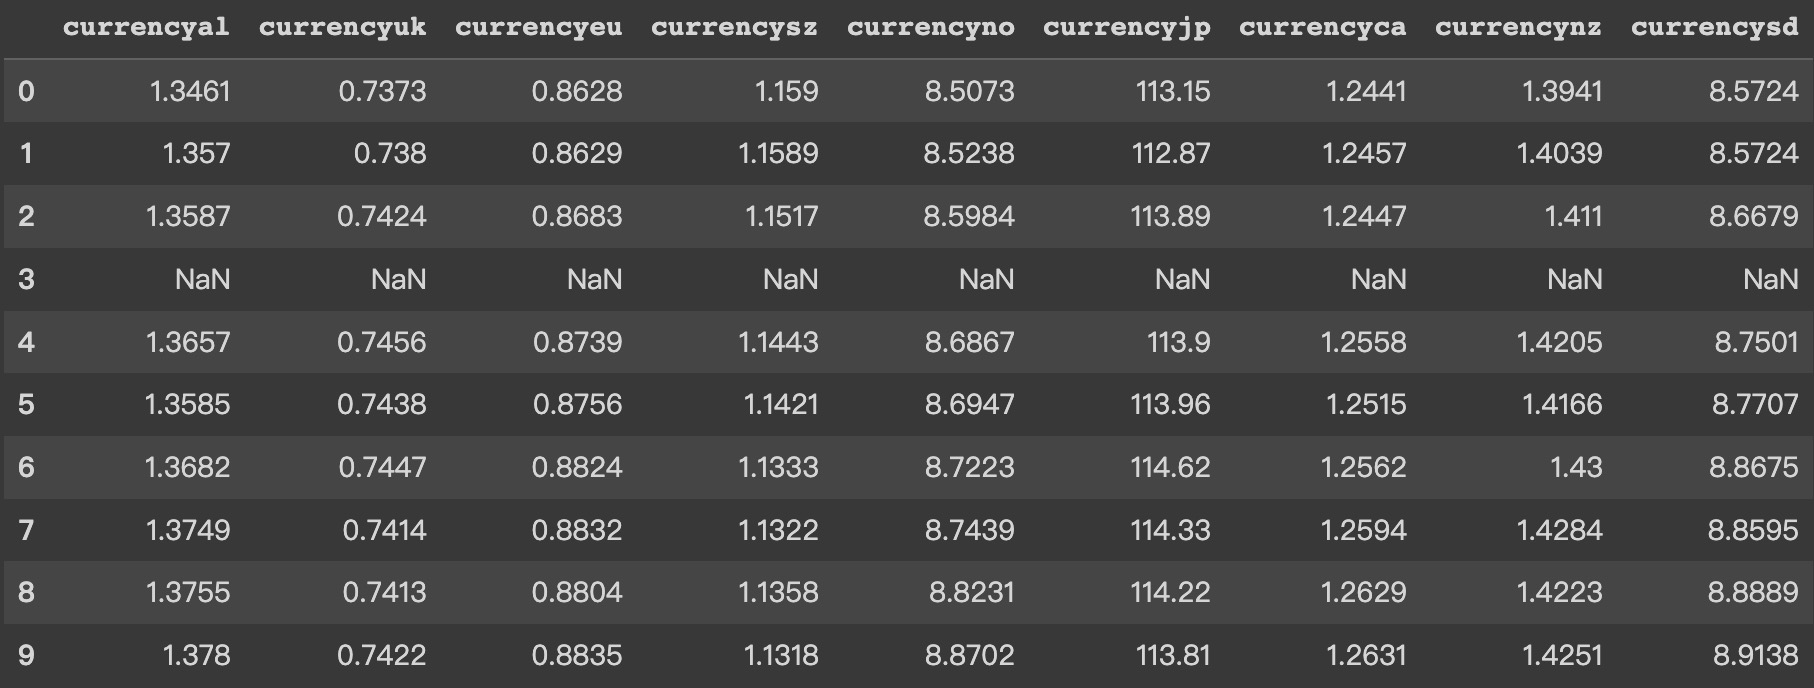
\includegraphics[scale=0.15]{Data.jpg} 
\end{slide}
}

% Part 2
\section{VaR Calculation}
\frame{
\begin{slide}
\centerslidesfalse
\frametitle{VaR Calculation}
\begin{description}
\item[Here we use three method to calculate VaR, they're given as follows:]
\end{description}
\begin{enumerate}
\item Historical VaR
\item Normal distribution Assumption
\item Monte Carlo Simulation
\end{enumerate}
\end{slide}
}

\frame{
\begin{slide}
  \frametitle{VaR Calculation-Historical VaR}
\begin{description}
\item[First we plot the historical return distribution.] 
\end{description}
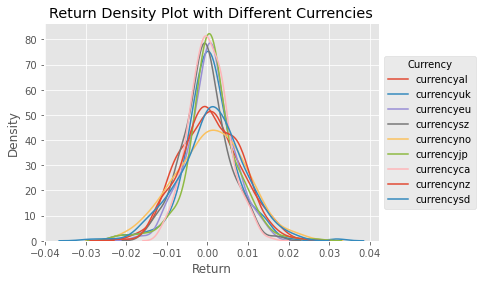
\includegraphics[scale=0.6]{return density.png} 
\end{slide}
}

\frame{
\begin{slide}
  \frametitle{VaR Calculation-Historical VaR}
\begin{description}
\item[Then we plot historical return.]
\end{description}
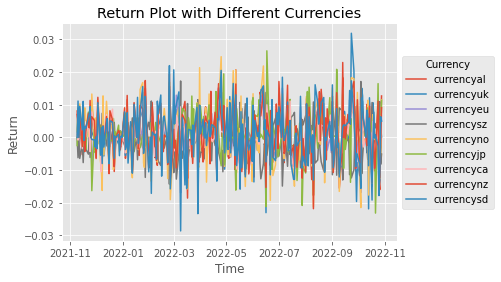
\includegraphics[scale=0.6]{return.png} 
\end{slide}
}

\frame{
\begin{slide}
\frametitle{VaR Calculation-Normal distribution Assumption}
\begin{description}
\item[Assume the currency return is normally distributed, we plot the] \item[normal distribution of the return for each currency.]
\end{description}
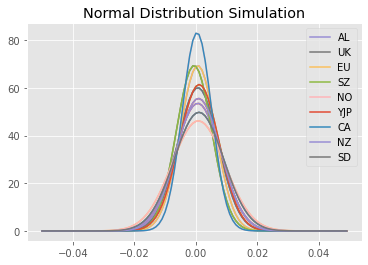
\includegraphics[scale=0.6]{ND simulation.png} 
\end{slide}
}

\frame{
\begin{slide}
\frametitle{VaR Calculation-Monte Carlo Simulation}
\begin{description}
\item[We simulate n path of the exchange rate and return, and then] \item[calculate the VaR of Monte Carlo Simulation Method.] 
\end{description}
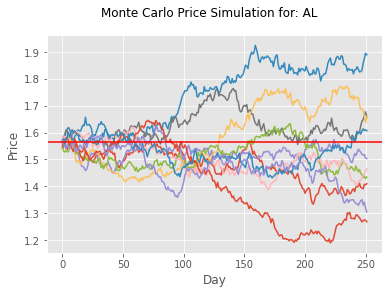
\includegraphics[scale=0.38]{MCSAL-P.png} 
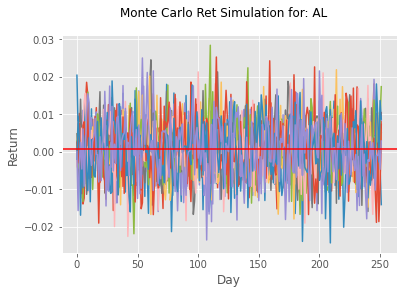
\includegraphics[scale=0.38]{MCSAL-R.png} 
\end{slide}
}

\frame{
\begin{slide}
\frametitle{VaR Calculation-Monte Carlo Simulation}
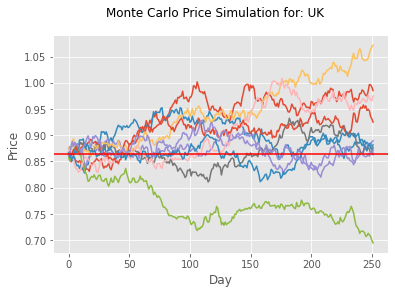
\includegraphics[scale=0.3]{MCSUK-P.png} 
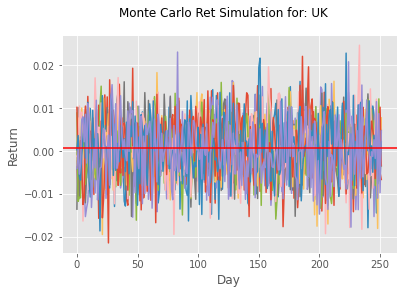
\includegraphics[scale=0.3]{MCSUK-R.png} 
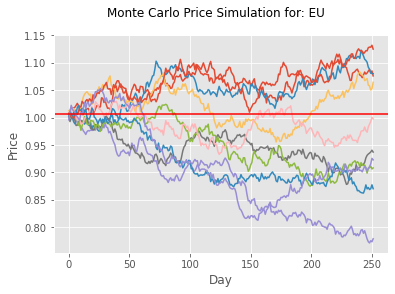
\includegraphics[scale=0.3]{MCSEU-P.png} 
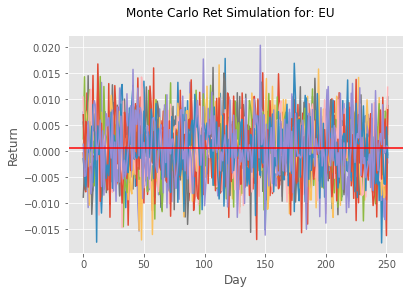
\includegraphics[scale=0.3]{MCSEU-R.png} 
\end{slide}
}

\frame{
\begin{slide}
\frametitle{VaR Calculation-Monte Carlo Simulation}
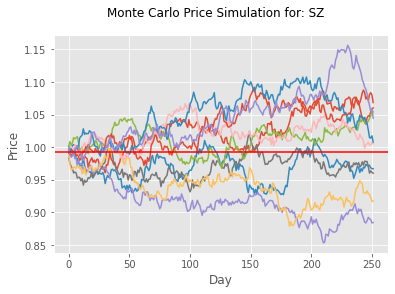
\includegraphics[scale=0.3]{MCSSZ-P.png} 
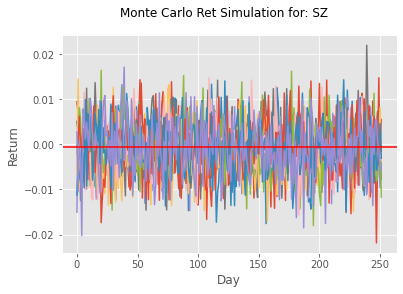
\includegraphics[scale=0.3]{MCSSZ-R.png} 
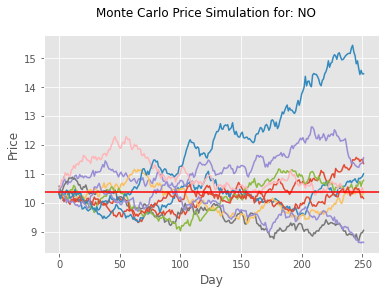
\includegraphics[scale=0.3]{MCSNO-P.png} 
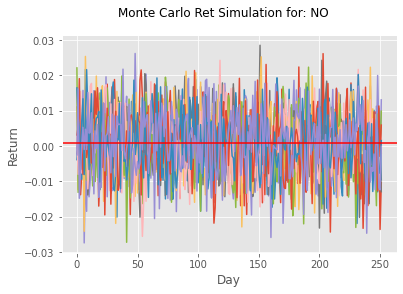
\includegraphics[scale=0.3]{MCSNO-R.png} 
\end{slide}
}

\frame{
\begin{slide}
\frametitle{VaR Calculation-Monte Carlo Simulation}
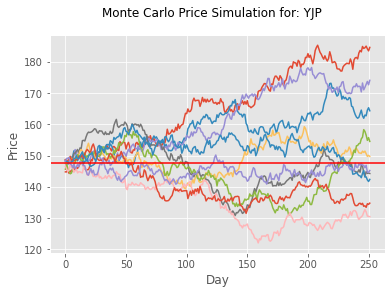
\includegraphics[scale=0.3]{MCSYJP-P.png} 
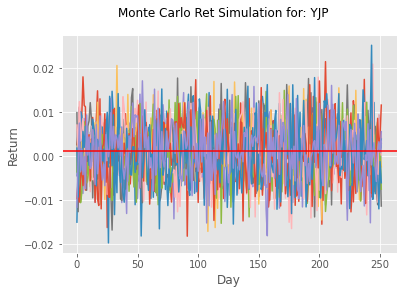
\includegraphics[scale=0.3]{MCSYJP-R.png} 
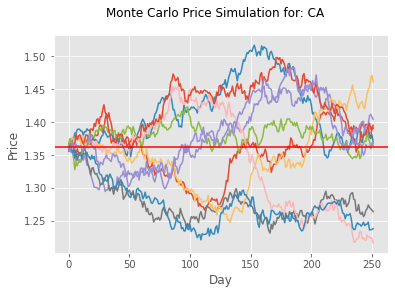
\includegraphics[scale=0.3]{MCSCA-P.png} 
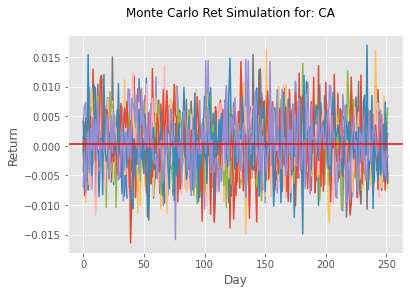
\includegraphics[scale=0.3]{MCSCA-R.png} 
\end{slide}
}

\frame{
\begin{slide}
\frametitle{VaR Calculation-Monte Carlo Simulation}
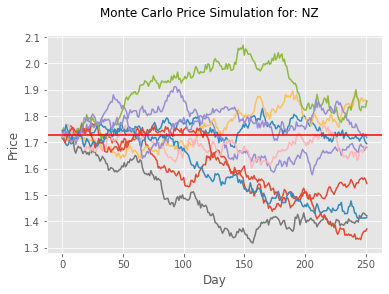
\includegraphics[scale=0.3]{MCSNZ-P.png} 
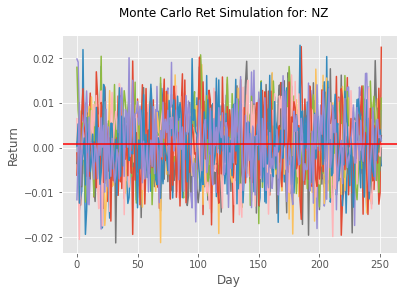
\includegraphics[scale=0.3]{MCSNZ-R.png} 
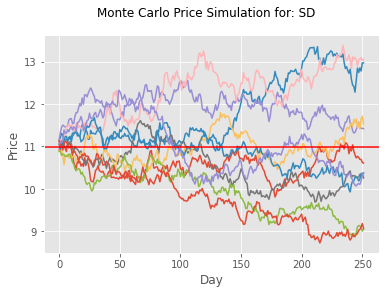
\includegraphics[scale=0.3]{MCSSD-P.png} 
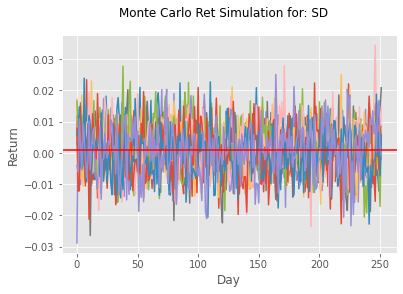
\includegraphics[scale=0.3]{MCSSD-R.png} 
\end{slide}
}

\frame{
\begin{slide}
\frametitle{VaR Calculation-Summary}
\begin{description}
\item[We set alpha value to 5, so we want to look at how much we]
\item[lose at a 5 percent of chance in one day. In all of the three]
\item[method, we see NO(Norwegian Krone)has the lowest VaR, thus]
\item[is relatively risky than other currencies.]
\end{description}
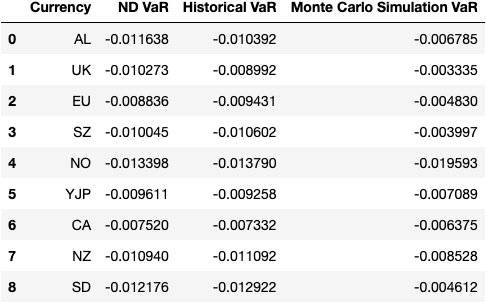
\includegraphics[scale=0.55]{VaR.jpg} 
\end{slide}
}

% Part 3
\section{Volatility Calculationa and Variance-Covariance Martix}
\frame{
\begin{slide}
  \centerslidesfalse
  \frametitle{Volatility Calculationa and Variance-Covariance Martix} 
\begin{description}
\item[We can also calculate volatility of return to measure the riskness]
\item[of the asset. From the result of the daily and annual volatility]
\item[calculated, we see currency yjp has the highest volatility. ]
\end{description}
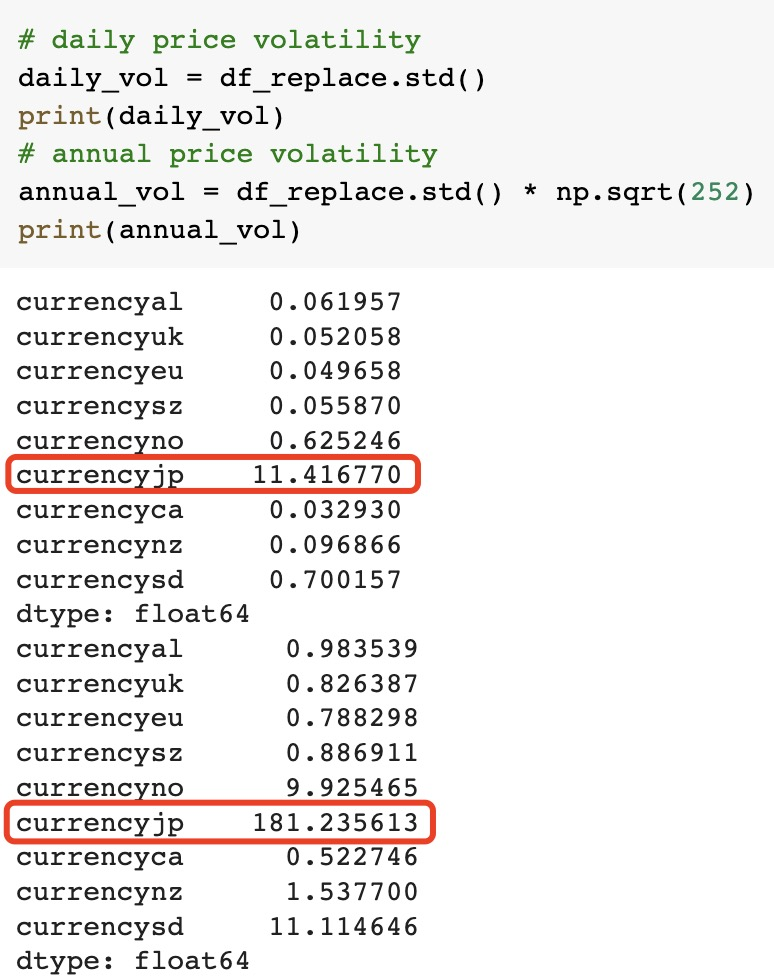
\includegraphics[scale=0.16]{Volatility.jpg} 
\end{slide}
}

\frame{
\begin{slide}
  \centerslidesfalse
  \frametitle{Volatility Calculationa and Variance-Covariance Martix} 
\begin{description}
\item[We can see all the G10 currencies' exchange to USD are highly]
\item[correlated, and Swiss Franc has a negative correlation with all]
\item[other currencies.]
\end{description}
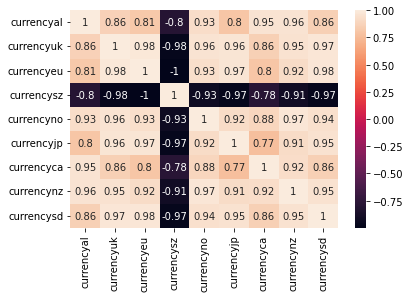
\includegraphics[scale=0.5]{matrix.png} 
\end{slide}
}
  
% Part 4
\section{Conclusion}
\frame{
\begin{slide}
\centerslidesfalse
\frametitle{Conclusion}

\begin{description}
\item[1.In all of the three VaR caculation method, we see NO]
\item[(Norwegian Krone) has the lowest VaR, thus is relatively ]
\item[risky than other currencies.]
\item[2.From the result of the daily and annual volatility calculated,]
\item[we see currency yjp has the highest volatility. ]
\item[3.it's hard to do risk diversification using only G10 currencies]
\item[since they are highly correlated, also the investor can use swiss]
\item[franc to hedge against risk.]
\end{description}
\end{slide}
}

\end{document}
